\chapter{Results}\label{chapter:results}
In this chapter, we present the results of our experiments.
First, the properties of the generated dataset are presented and visualized.
Then, the results of the different retrieval methods are presented and compared.
Finally, the results of ranking the LLM answers are presented and the influence of the different prompting strategies, model sizes, pre training methods and question types are discussed.

\section{Dataset}
Our dataset is constructed according to the procedure described in section \ref{sec:dataset}.
We now go more in depth on the properties of the final dataset, considering the type of queries, the number of answers per query and the length of the answers.
\\
The total number of queries in the final dataset is 50, each of which is accompanied by between 39 and 249 answers.
The number of answers depends on how many of the given answer in the base dataset by \cite{goeuriot:2021} were, still available, i.e. not from Reddit or Twitter.
Since this was not the same for all queries, the number of answers per query varies.
On average, there are about 178 evaluated documents per query available.

\subsection{Queries}
We identify two different query types in the dataset: questions and keyword queries.
Questions are queries that are formulated as a question, e.g. ``Is a ketogenic diet suitable for people with diabetes?'', while keyword based queries are more in the style of search engine queries, e.g. ``keto diet diabetes''.
\begin{table}[tb]
\centering
\begin{tabularx}{\textwidth}{XX}
\hline
\textbf{Keyword-Based Queries} & \textbf{Question-Type Queries} \\
\hline
best apps daily activity exercise diabetes & What are the most common chronic diseases? \\
\hline
my risk for developing type 2 diabetes & Is a ketogenic / keto diet suitable for people with diabetes? \\
\hline
multiple sclerosis stages phases & Can diabetes be cured? \\
\hline
\end{tabularx}
\caption{Samples of Keyword vs Question Type Queries}
\label{table:querie-samples}
\end{table}
Table \ref{table:querie-samples} shows some examples of the two query types.
Query topics are diverse, ranging from general queries about chronic diseases to specific questions about the suitability of certain diets for people with diabetes.
\\\\
\begin{figure}
\centering
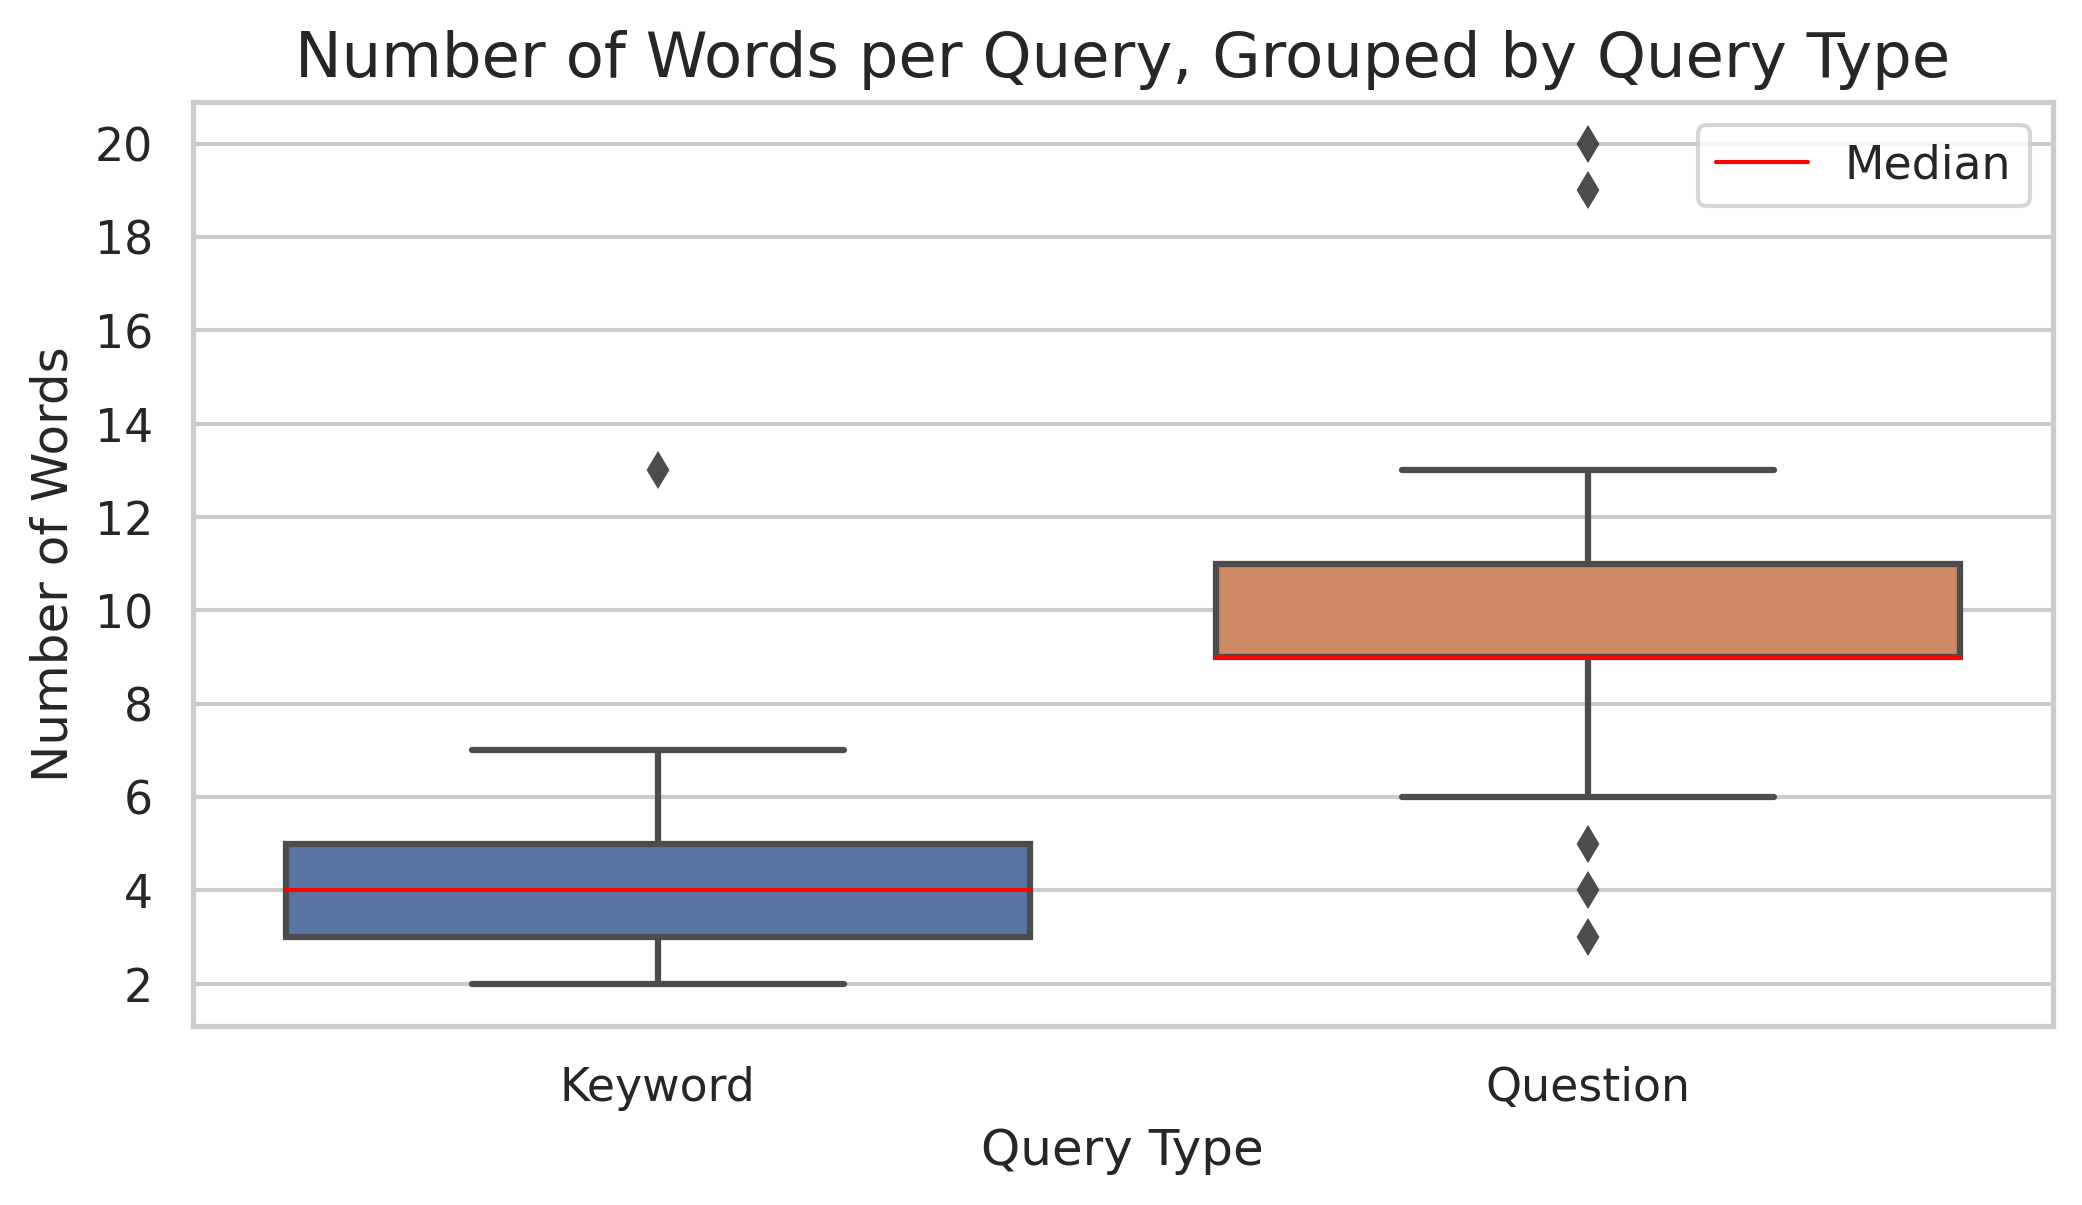
\includegraphics[width=\textwidth]{images/num_words_per_query.png}
\caption{Boxplot of the number of words per query, split by query type. Keyword queries are shorter than question queries with a median of 4 words compared to 7 words for the question queries.}
\label{fig:num_words_per_query}
\end{figure}
In total, we identify 17 question-style queries and 33 keyword-style queries.
Figure \ref{fig:num_words_per_query} shows the number of words per query for both query types.
As expected, the keyword queries are shorter than the question queries, with a median of 4 words compared to 7 words for the question queries.
The shortest query is only two words long, while the longest query is 20 words long.
In a later section, we investigate the differences in the performance of the different models depending on the two query types.
\subsection{Documents}
\begin{table}[tb]
\centering
\begin{tabular}{ll}
\hline
\textbf{Domain} & \textbf{Occurrences} \\
\hline
www.healthline.com & 603 \\
www.nationalmssociety.org & 419 \\
www.ms.org.au & 198 \\
jhu.pure.elsevier.com & 191 \\
www.msif.org & 183 \\
www.psychologytoday.com & 161 \\
www.urotoday.com & 155 \\
www.news-medical.net & 150 \\
www.sleepfoundation.org & 141 \\
www.aafp.org & 139 \\
\hline
\end{tabular}
\caption{Top 10 Most Frequently Occurring Domains}
\label{tab:top_domains}
\end{table}
The documents in the dataset are scraped from a total of 234 different domains.
Table \ref{tab:top_domains} shows the top 10 most frequently occurring domains in the dataset.
Most domains are health related, belonging to either health organizations, medical journals or health news websites.
Some domains are more general, e.g. there are also wikipedia.org pages in the dataset, as well as some domains from essay writing or homework help websites.
A total of 133 domains show up less than 10 times in the dataset, while 44 domains show up only once.
\\\\
\begin{figure}[tb]
\centering
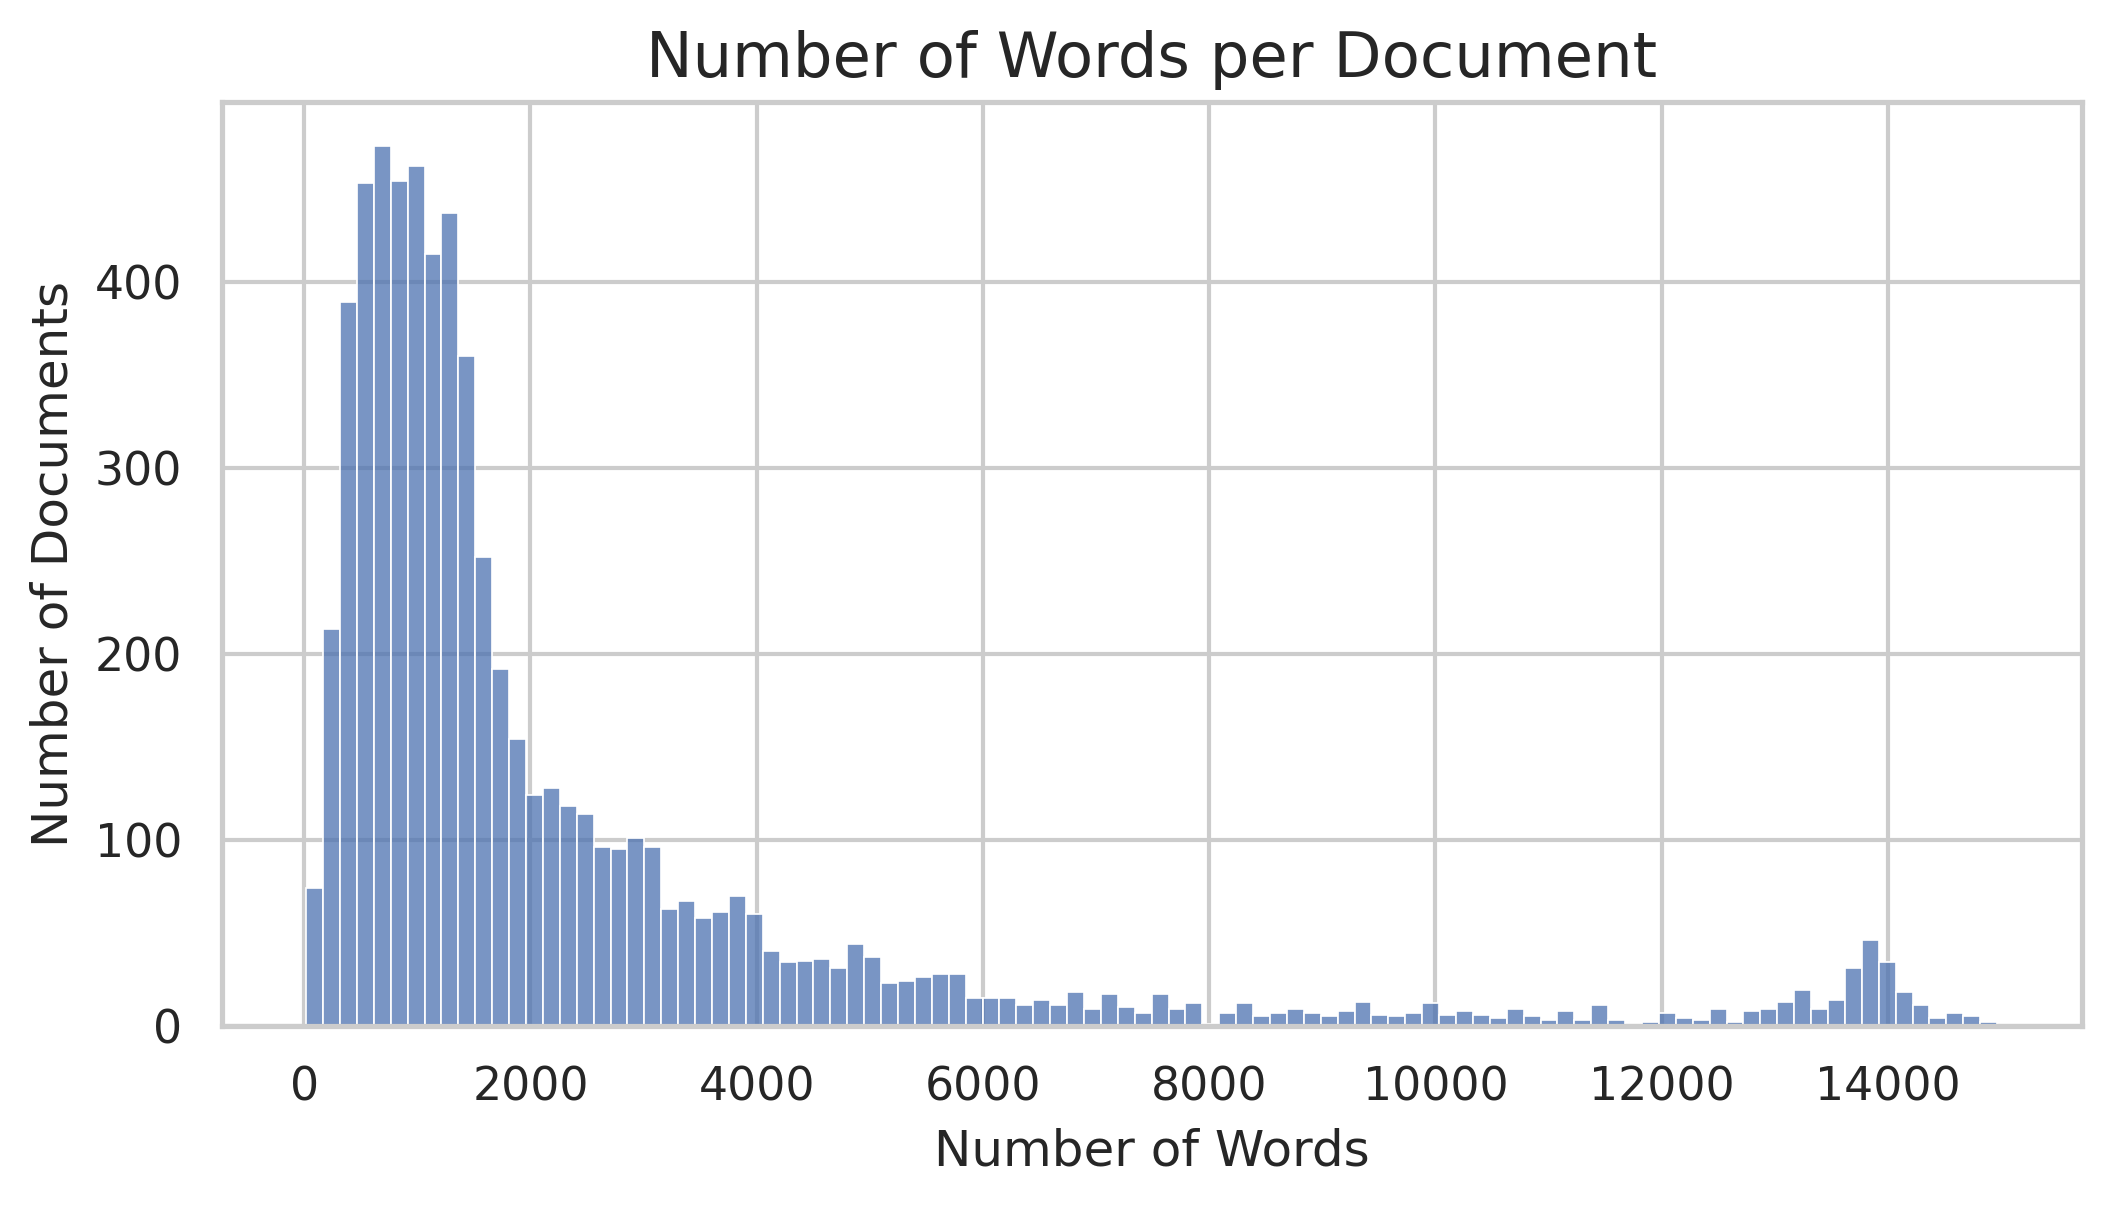
\includegraphics[width=\textwidth]{images/num_words_per_passage.png}
\caption{Histogram of the number of words per document. The plot is cut at 15 000 words, which excludes 120 or 2\% of the documents. The median number of words per document is 1354, while the mean is 2901.}
\label{fig:num_words_per_document}
\end{figure}
After preprocessing, the documents are cleaned of all HTML tags and of HTML elements containing fewer than 50 characters.
Figure \ref{fig:num_words_per_document} shows that the number of words per document is very high, with a median of 1354 words and a mean of 2901 words.
This is natural for documents scraped from the web, which do not only contain the main text, but also navigation bars, footers, sidebars and other elements.
Those can not be fully removed with our trivial preprocessing methods.
\subsection{Document Ratings}
The document metrics in the dimensions of readability, credibility and relevance are the human annotations from \cite{goeuriot:2021}.
Documents can have multiple ratings for each dimension, if they are annotated for multiple queries.
This means that the total number of ratings per dimension (8902) is higher than the number of documents in the dataset (6692).
\\

In general, a surprisingly high number of documents are rated as not relevant to the given query.
Figure \ref{fig:heatmap_rel_cred_read} shows three heatmaps, with each relevance category being displayed in its own heatmap.
Documents rated with 0 relevance make up nearly half of the dataset and generally have lower credibility and readability scores.
The most relevant documents are generally also the most credible and readable ones.
The correlation between relevance and credibility is only 0.08, so while it is slightly positive, it is not very strong.
For readability and relevance, the correlation is 0.22, which is slightly stronger, but still does not show a strong connection.
This can be interpreted as the relevance of a document being independent of its credibility and readability, which shows that the annotators were able to judge the relevance of a document independently of its credibility and readability.
\begin{figure}
\centering
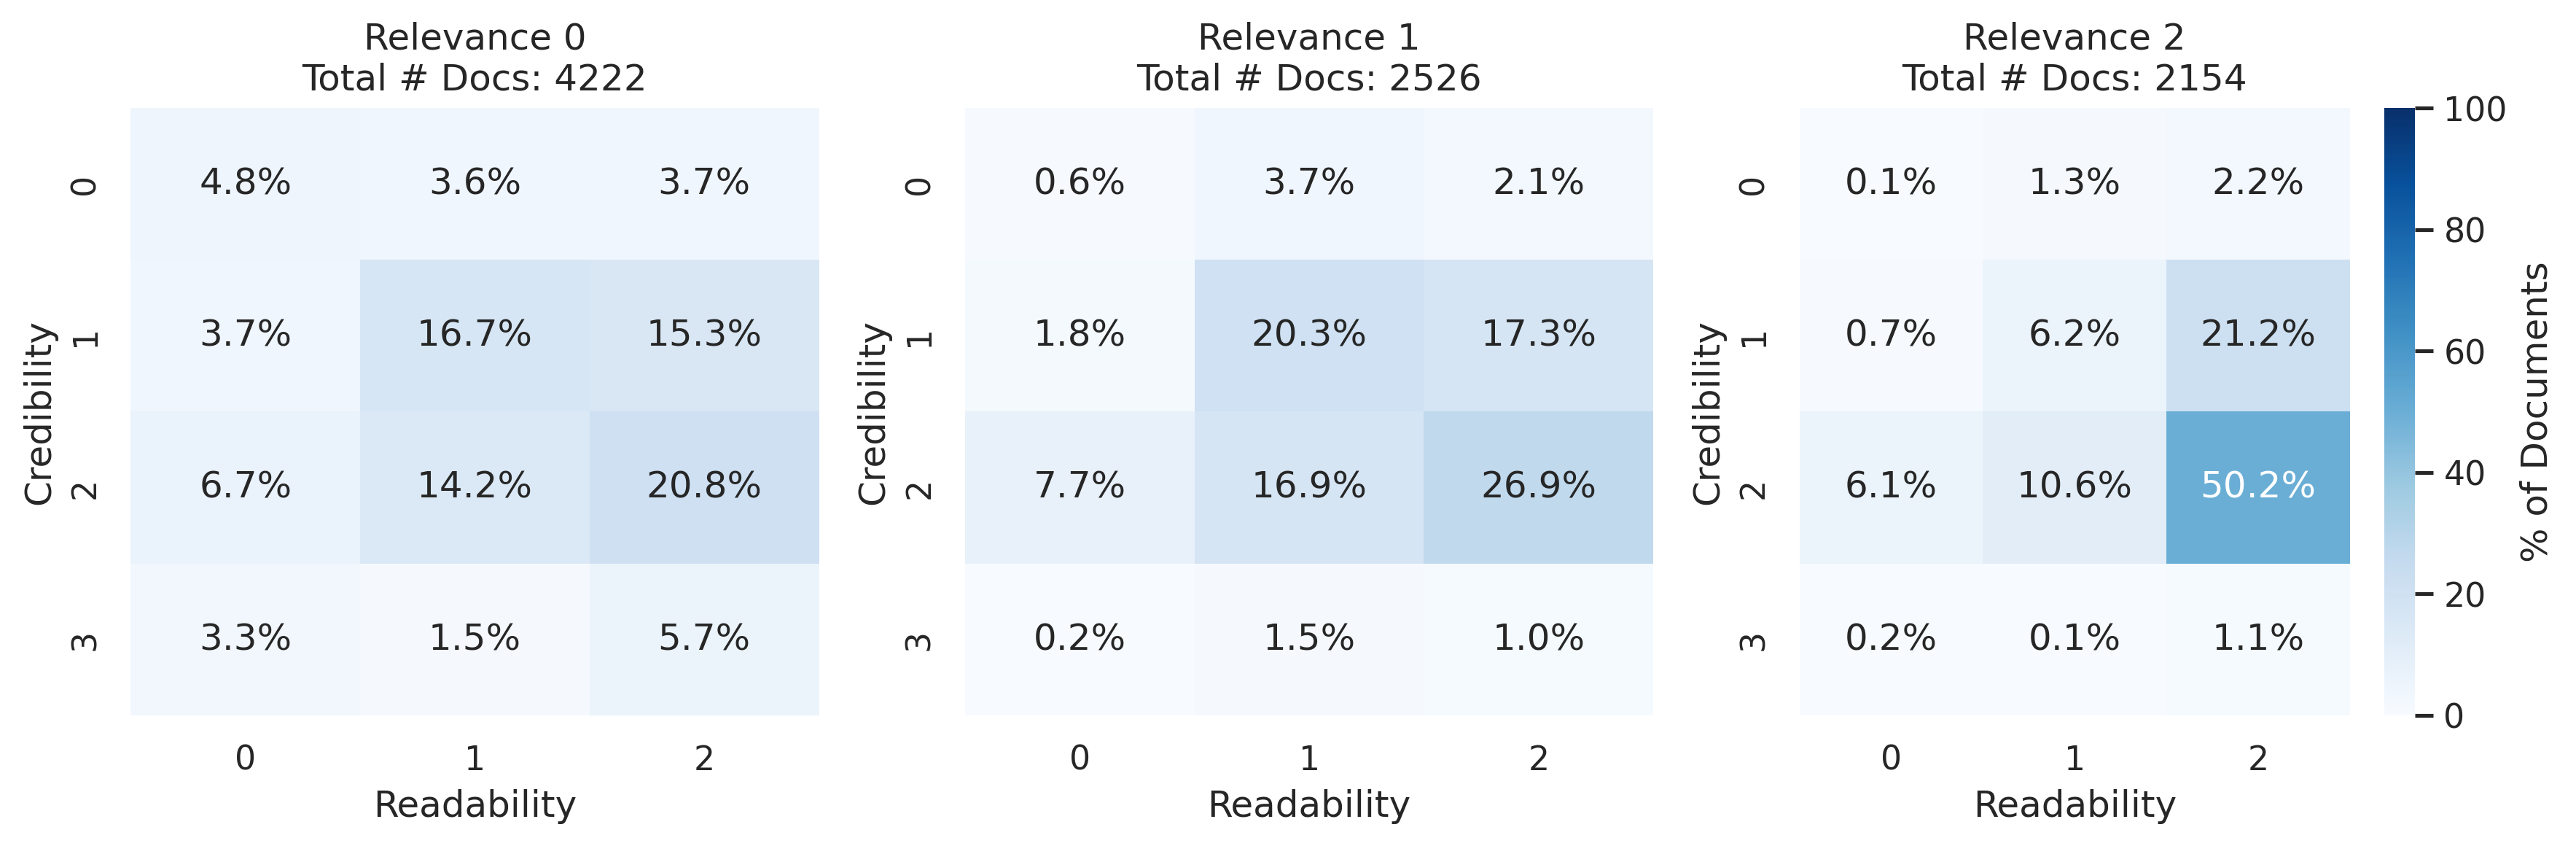
\includegraphics[width=\textwidth]{images/heatmap_qrels.png}
\caption{Three heatmaps, one for each relevance category, plotting credibility against readability.
The total number of documents with the given relevance ranking is in the title of the heatmap.
In all three heatmaps, the highest number of documents is concentrated in the range between 1 and 2 for both credibility and readability, with 2 credibility and 2 readability being the most common combination.
}
\label{fig:heatmap_rel_cred_read}
\end{figure}

\subsection{Documents with Ratings for Multiple Queries}
As mentioned previously, some documents have multiple ratings for different queries.
In total 875 documents are rated for multiple queries, with the highest number of individual annotations for a single document being 18.
Documents with multiple ratings are often general articles about a certain topic, e.g. ``What is Multiple Sclerosis?''.
Those are then retrieved for multiple queries that focus on different aspects of the topic, e.g. ``List of multiple sclerosis symptoms'' and ``Can I pass multiple sclerosis to other family members?''.
As expected, the different relevance ratings for the same document are often different, since the relevance of a document depends on the query.
Interestingly, we also find that the credibility and readability ratings for the same document can be different.
In Appendix \ref{appendix:dataset}, we show an example of a document with multiple ratings for different queries.
The 15 different ratings cover nearly all possible combinations of relevance, credibility and readability.
\\
As all documents for one query are annotated by the same person according to \cite{goeuriot:2021}, we assume that the annotators were consistent in their ratings for the same query.
Because we are only interested in the ranking of the documents for one query at a time, we do not remove or aggregate the scores, as this could alter the ranking of the documents compared to documents that were only ranked for this specific query.

\section{Retrieval Pipelines}
In this section, we present the results of the different retrieval pipelines.
We chose to evaluate the pipelines using nDCG@10, which was explained in section \ref{sec:evaluation-of-retrieval-models}.
nDCG is a suitable metric for our task, as it takes into account multiple different relevance/credibility/readability levels instead of only the binary relevant/not relevant distinction.
Furthermore, it emphasizes the importance of the top results, which we expect to be the most competitive ones against the LLM answers, so it is important to be able to distinguish between at the top level.
We chose a cutoff of 10, because even tough the minimum available number of answers per query is 39, the number of relevant results is much lower.
\\
\subsection{Baseline Pipelines}
Our baseline retrieval pipelines are the TF-IDF and BM25 pipelines, each once with and once without query expansion.
\begin{table}[tb]
\centering
\begin{tabularx}{\textwidth}{lXXX}
Pipeline    & Relevance          & Readability        & Credibility        \\ \hline
DPH         & \textbf{0.643} & 0.742 & 0.539 \\
DPH\ (qe)     & 0.637 & \textbf{0.751} & 0.51  \\
TF-IDF     & 0.64  & 0.746 & 0.551 \\
TF-IDF (qe) & 0.636 & \textbf{0.751} & \textbf{0.557}
\end{tabularx}
\caption{Results of the baseline pipelines, shown as nDCG@10. Query expansion is denoted by qe.
All pipelines perform similarly, the influence of query expansion is small.}
\label{tab:baseline_pipelines}
\end{table}
Table \ref{tab:baseline_pipelines} shows the results of the baseline pipelines.
Performance on all three metrics is similar for all pipelines.
The rankings seem to be closest to the human readability ranking, scoring around 0.75 for all pipelines.
Relevance is interestingly lower than that, with scores around 0.64.
Since those models are designed to retrieve relevant documents, we would expect the relevance scores to be higher.
The credibility scores are the lowest, with scores around 0.55.
The models do not have any mechanics for assessing credibility, so this is not surprising.

\subsection{Transformer Pipelines}
\begin{table}[tb]
\centering
\begin{tabularx}{\textwidth}{lXXX}
Pipeline    & Relevance          & Readability        & Credibility        \\ \hline
Best baseline    & 0.643 & 0.751 & 0.557 \\
colbertv1      & 0.626 & 0.774 & 0.633 \\
colbertv2       & 0.634 & 0.799 & 0.65  \\
duoT5            & 0.64  & 0.805 & 0.714 \\
monoT5           & \textbf{0.645} & \textbf{0.813} & \textbf{0.722}
\end{tabularx}
\caption{Results of the transformer pipelines, shown as nDCG@10. Best results of the baseline pipelines are shown for comparison. All models are trained on the MS MARCO passage ranking dataset(\cite{bajaj:2016}).}
\label{tab:transformer_pipelines}
\end{table}
Table \ref{tab:transformer_pipelines} shows the nDCG@10 scores for the different transformer-based pipelines, compared to the best baseline results.
The monoT5 pipeline performs best on all three metrics, with scores of 0.645 for relevance, 0.813 for readability and 0.722 for credibility.
Re-ranking the top 10 results using duoT5 made the results slightly worse.
ColBERTv2 shows a slight improvement over ColBERTv1, but is still worse in relevance, while being better in readability and credibility.
\\\\
In general, the transformer-based models perform very similar to the baseline models in terms of relevance, but all transformer-based models achieve higher scores on readability and credibility.
We attribute this to the fact that the transfomer-based models do not consider the documents as bags of words, but instead use the full text of the documents.
This is especially important for readability, as the models can now take into account the structure of the text, including stopwords, punctuation and other elements that are removed for the baseline models.
Even tough the transformer models are not specifically trained to consider readability and credibility, the relevant passages in the MS MARCO corpus seem to reflect those properties.

\subsection{External Document Scores}
Because ranking models that consider readability the main ranking dimension are not available, we investigate adding external scores to the ranking process.
First, the statistical scores described in Section \ref{sec:external-scores} are calculated for all documents in the dataset.
We then compare the calculated scores to the readability scores assigned by the human annotators.
Unfortunately, for our dataset we do not find a strong correlation between the readability scores and the statistical scores.
The Flesch Reading Ease score has a correlation of 0.177 with the readability scores, while the full textstat score has a slightly negative correlation of -0.147.
Those correlations are not strong enough to justify using the statistical scores as a proxy for readability.
\\
This probably is connected to the fact that the documents in our dataset are scraped from the web, which means that even after preprocessing they still contain noise, which is not accounted for by the statistical scores.

\section{Ranking of Generated Answers}
We now present the results of ranking the LLM answers using the best performing pipeline, the monoT5 pipeline.
Because monoT5 performs best on all three metrics, we use it for all further experiments and only evaluate the one ranking produced by this pipeline.
\\
In total, we rank 16000 generated answers, with each of the 8 models generating 10 answers for each of the 4 different prompting strategies for all 50 queries.
\begin{figure}
\centering
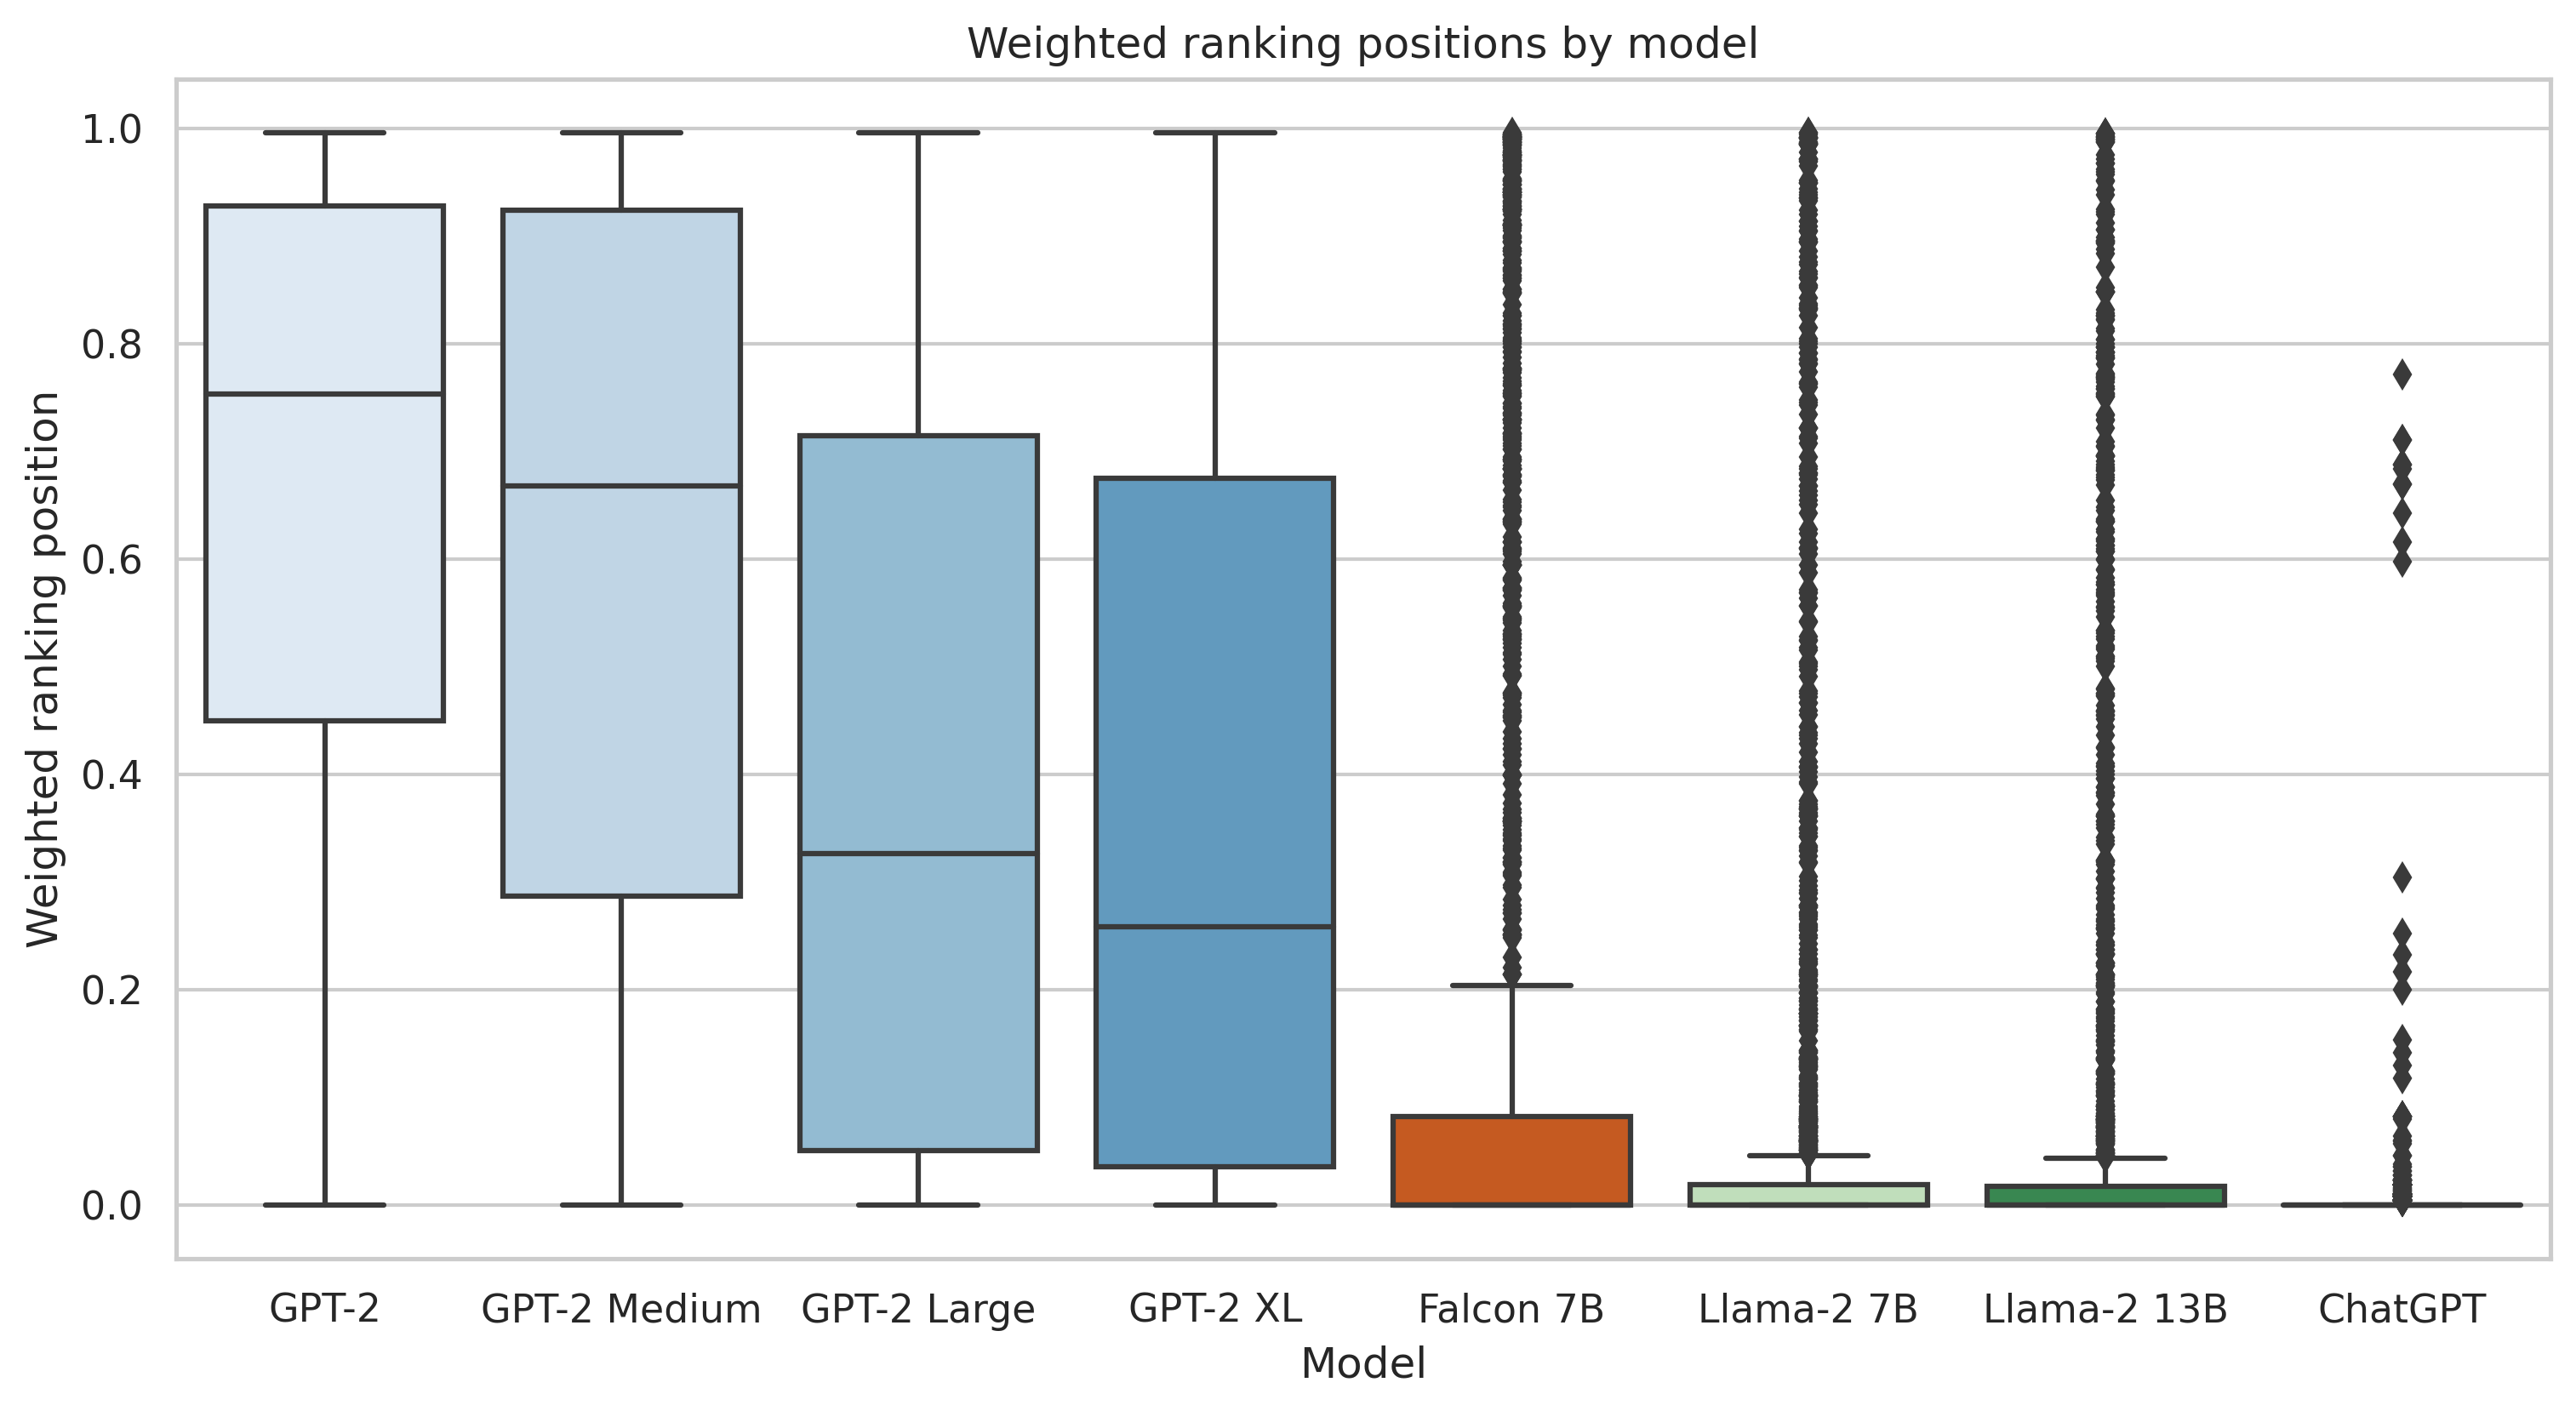
\includegraphics[width=\textwidth]{images/weighted_position_boxplot.png}
\caption{Boxplot of the normalized position of the LLM answers, by model. }
\label{fig:weighted_position_boxplot}
\end{figure}
Figure \ref{fig:weighted_position_boxplot} shows the normalized position of the LLM answers in the ranking.
The normalized position is the absolute position of the answer in the ranking, divided by the total number of documents for the query.
\\
The GPT-2 models generally perform worse, which was expected, as they are not fine-tuned for the task of question answering and are generally much smaller than the other models.
Interestingly, even those models have a significant number of first place rankings.
The four different sizes of GPT-2 nicely show the effect of model size on ranking performance, with the median ranking position improving significantly with each size increase.
\\
Of the fine-tuned models, ChatGPT performs best with a median position of 0.006, scoring the best or second-best answer at nearly all queries.
Falcon 7B is the worst of the fine-tuned models with the Llama models performing slightly better.
This could potentially be due to the more sophisticated fine-tuning techniques for the Llama models, which are described in section \ref{sec:dialog-models}.
Between the two Llama models, the smaller one is slightly better, but they perform very similar.
This is not consistent with other benchmarks, where the larger model usually performs better, as shown in the following subsection \ref{sec:benchmark_comparison}.
\\
ChatGPT is also the most consistent model, with the smallest standard deviation of 0.05.
The other models have much higher standard deviations, with the Llama models both being around 0.2 and the other models between 0.3 and 0.35.
\\

\subsection{Influence of Prompting Strategy}
The different prompting strategies strongly influence the final rankings of the LLM answers.
\begin{table}[tb]
\centering
\begin{tabular}{lcccc}
\textbf{Model}        & \textbf{No Prompt} & \textbf{QA}     & \textbf{QuestionAnswer} & \textbf{MultiMedQA} \\\hline
GPT-2        & 0.763      & 0.663 & 0.614    & 0.603      \\
GPT-2 Medium & 0.675      & 0.524 & 0.544    & 0.618      \\
GPT-2 Large  & 0.496      & 0.393 & 0.336    & 0.374      \\
GPT-2 XL     & 0.509      & 0.336 & 0.327    & 0.292      \\
Falcon 7B    & 0.324      & 0.133 & 0.118    & 0.012      \\
Llama-2 7B   & 0.211      & 0.073 & 0.027    & 0.005      \\
Llama-2 13B  & 0.218      & 0.068 & 0.032    & 0.01       \\
ChatGPT      & 0.006      & 0.01  & 0.007    & 0.001     
\end{tabular}
\caption{Mean normalized position of the LLM answers, by prompting strategy.
The prompting strategies are described in section \ref{sec:prompting-approaches}, order here from least to most complex.
Increasing prompting complexity generally improves the ranking of the LLM answers for most models, with exception of GPT-2 Medium and GPT-2 Large.
}
\label{tab:prompting_strategy}
\end{table}
Table \ref{tab:prompting_strategy} shows the mean normalized position of the LLM answers for the different prompting strategies.
Starting with no prompt produces the worst ranking results for all models, except for ChatGPT where the QuestionAnswer prompt performs slightly worse.
The rankings improve with each more complex prompting strategy, except for GPT-2 Medium and GPT-2 Large, which perform best on the QA and the QuestionAnswer prompts respectively.
Even the three smaller instruction tuned models (Falcon and Llama) show strong improvements when going from no prompt at all to the simple QA prompt.
As those models are already fine-tuned on the task of question answering, we could have expected them to perform better on the no prompt strategy.
The biggest model, ChatGPT, shows the smallest differences in scores between the different prompting strategies, but still performs best with the MultiMedQA prompt.
\\
The results are consistent with the findings by \cite{reynolds:2021} that more complex prompting strategies improve the performance of LLMs.

\subsection{Keyword vs Question Queries}
\begin{figure}
    \centering
    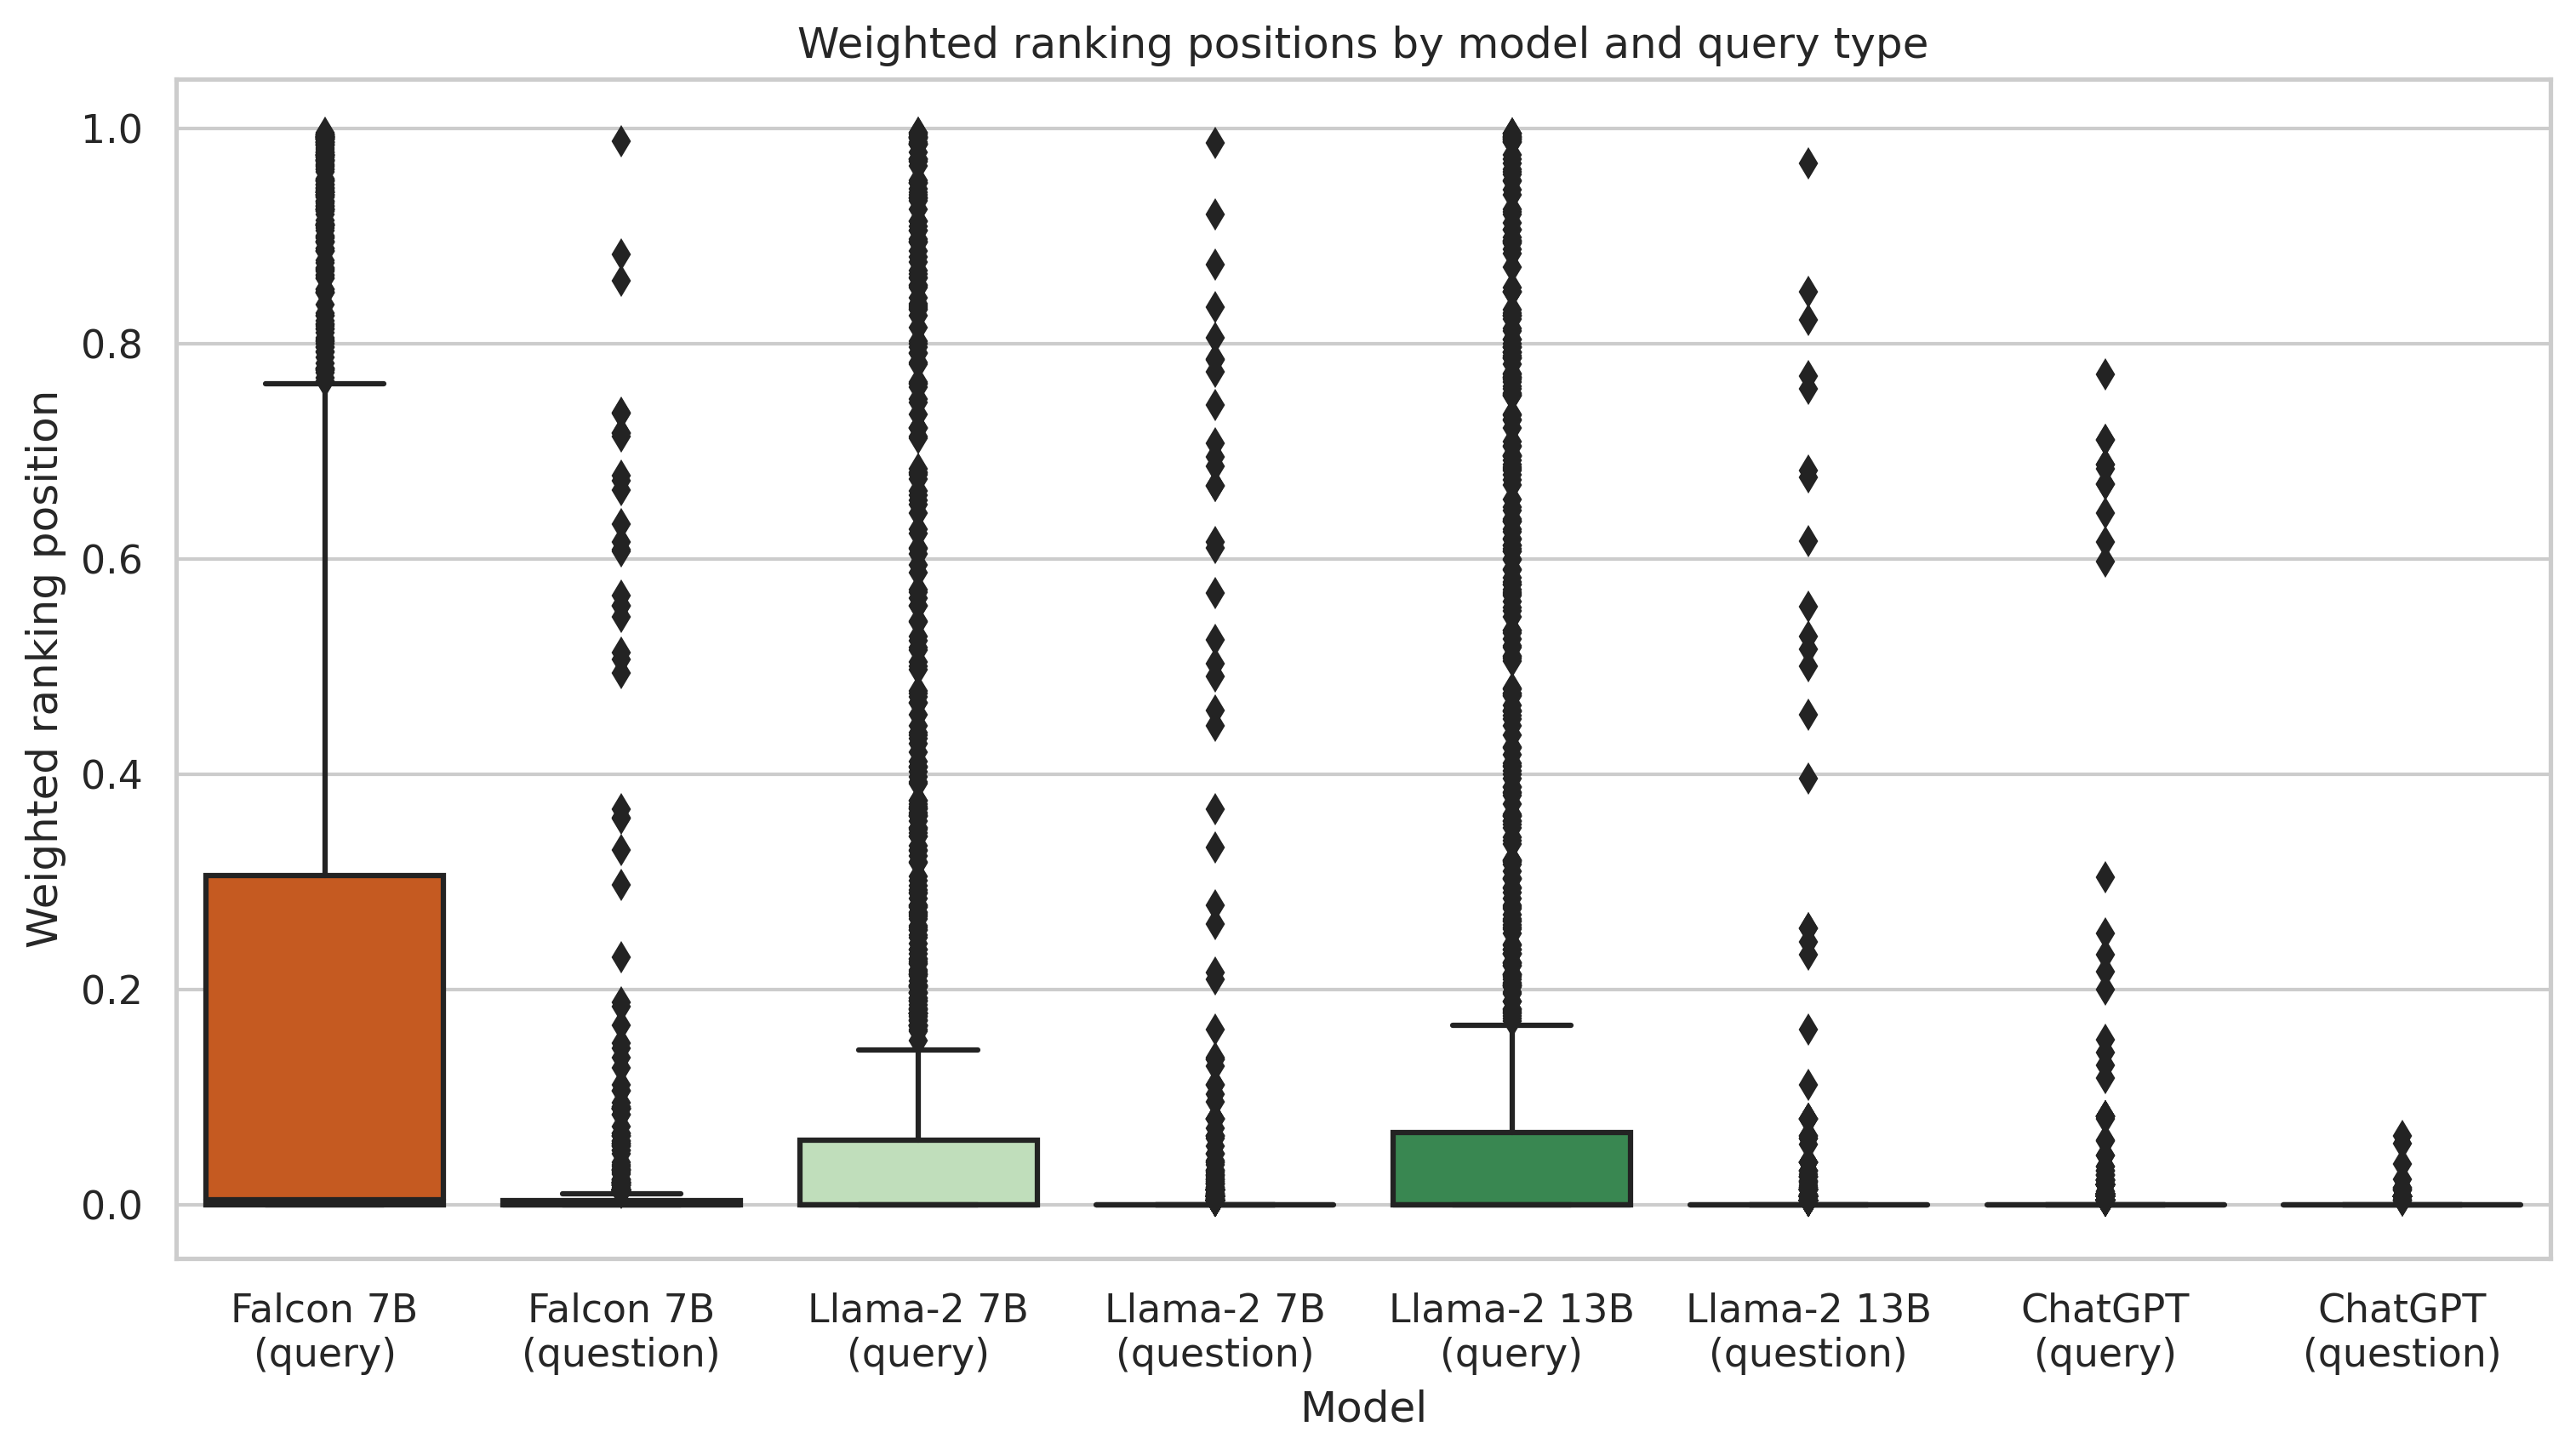
\includegraphics[width=\textwidth]{images/weighted_position_boxplot_by_model_and_question.png}
    \caption{Boxplot of the normalized position of the LLM answers, by model and query type.}
    \label{fig:weighted_position_boxplot_by_model_and_question}
\end{figure}
Figure \ref{fig:weighted_position_boxplot_by_model_and_question} shows the normalized position of the LLM answers, split by query type and model.
Answers generated for the properly phrased question-type queries achieve higher median rankings than the answers generated for the keyword queries.
The spread of the rankings is also smaller for the question-type queries, with the keyword queries having more outliers at the bottom of the ranking.
This also holds true for ChatGPT, which is the most consistent model overall.
\\


\subsection{Comparison to other Benchmarks}\label{sec:benchmark_comparison}
We compare the median normalized ranking position of the LLM answers to the results of other benchmarks.
To our knowledge, there are currently no benchmarks available that evaluate the performance of LLMs for long form question answering and provide results for the same models that we use.
The HuggingFace Open LLM Leaderboard by \cite{beeching:2023} provides results for many models hosted on the HuggingFace hub, over multiple different benchmarks.
From here, we select the ARC~(\cite{clark:2018}), the HellaSwag~(\cite{zellers:2019}) and the MMLU~(\cite{hendrycks:2020}) benchmarks, which are all single choice question answering benchmarks.
\begin{table}[tb]
    \centering
    \begin{tabularx}{\textwidth}{lcccc}
    \textbf{Model} & \textbf{Mean Ranking} & \textbf{ARC}  & \textbf{HellaSwag} & \textbf{MMLU} \\\hline
    GPT-2          & 0.661                             & 21.8          & 31.6               & 25.9          \\
    GPT-2 Medium   & 0.59                              & 27.0          & 40.2               & 26.6          \\
    GPT-2 Large    & 0.4                               & 25.9          & 45.6               & 26.1          \\
    GPT-2 XL       & 0.366                             & 30.3          & 51.4               & 26.4          \\
    Falcon 7B      & 0.147                             & 46.2          & 70.9               & 25.8          \\
    Llama-2 13B    & 0.082                             & 59.0          & 81.9               & 54.6          \\
    Llama-2 7B     & 0.079                             & 52.9          & 78.6               & 48.3          \\
    ChatGPT        & \textbf{0.006}                    & \textbf{85.2} & \textbf{85.5}      & \textbf{70.0}
    \end{tabularx}
    \caption{Comparison of the mean normalized ranking position of the LLM answers to the results of other benchmarks.
    For the HuggingFace models, those scores are taken from the HuggingFace Open LLM Leaderboard by \cite{beeching:2023}.
    For ChatGPT, we estimate the score from the GPT-4 Technical Report~(\cite{openai:2023}), which provides scores for GPT-3.5, the underlying model of ChatGPT.
    This is not the exact model we use in out testing, but we assume that the performance is similar.
    Mean Ranking is the mean normalized ranking position over all generated answers for the model.
    }
    \label{tab:benchmark_comparison}
\end{table}
Table \ref{tab:benchmark_comparison} shows the scores over those benchmarks, as well as the mean normalized ranking position of the LLM answers.
On all benchmarks, there is the general trend of higher number of model parameters leading to better scores.
For our dataset this trend is only broken for the two Llama versions, with the 7B model ranking slightly better than the 13B model.
Other than that, our results are consistent with the results of the other benchmarks.

